\subsection{Basics}
\begin{frame}{\insertsection} % instead of the section, you can title frames whatever you want. for the first frame of a section, this here is really new though
	\framesubtitle{\insertsubsection} % you have to set the subtitle `manually' unfortunately
	\begin{itemize}[<+->] % reveals one point at a time
		\item This is a basic itemization
		\item Only one point at a time
		\item Even \pause pauses \pause in midsentence and \pause points. % pause for manual pause
    \end{itemize}
    \pause \textbf{Everything looks neat and simple.}
\end{frame}

\subsection{Some more}
\begin{frame}{\insertsection}
	\framesubtitle{\insertsubsection}
	\begin{figure}[h]
		\centering
		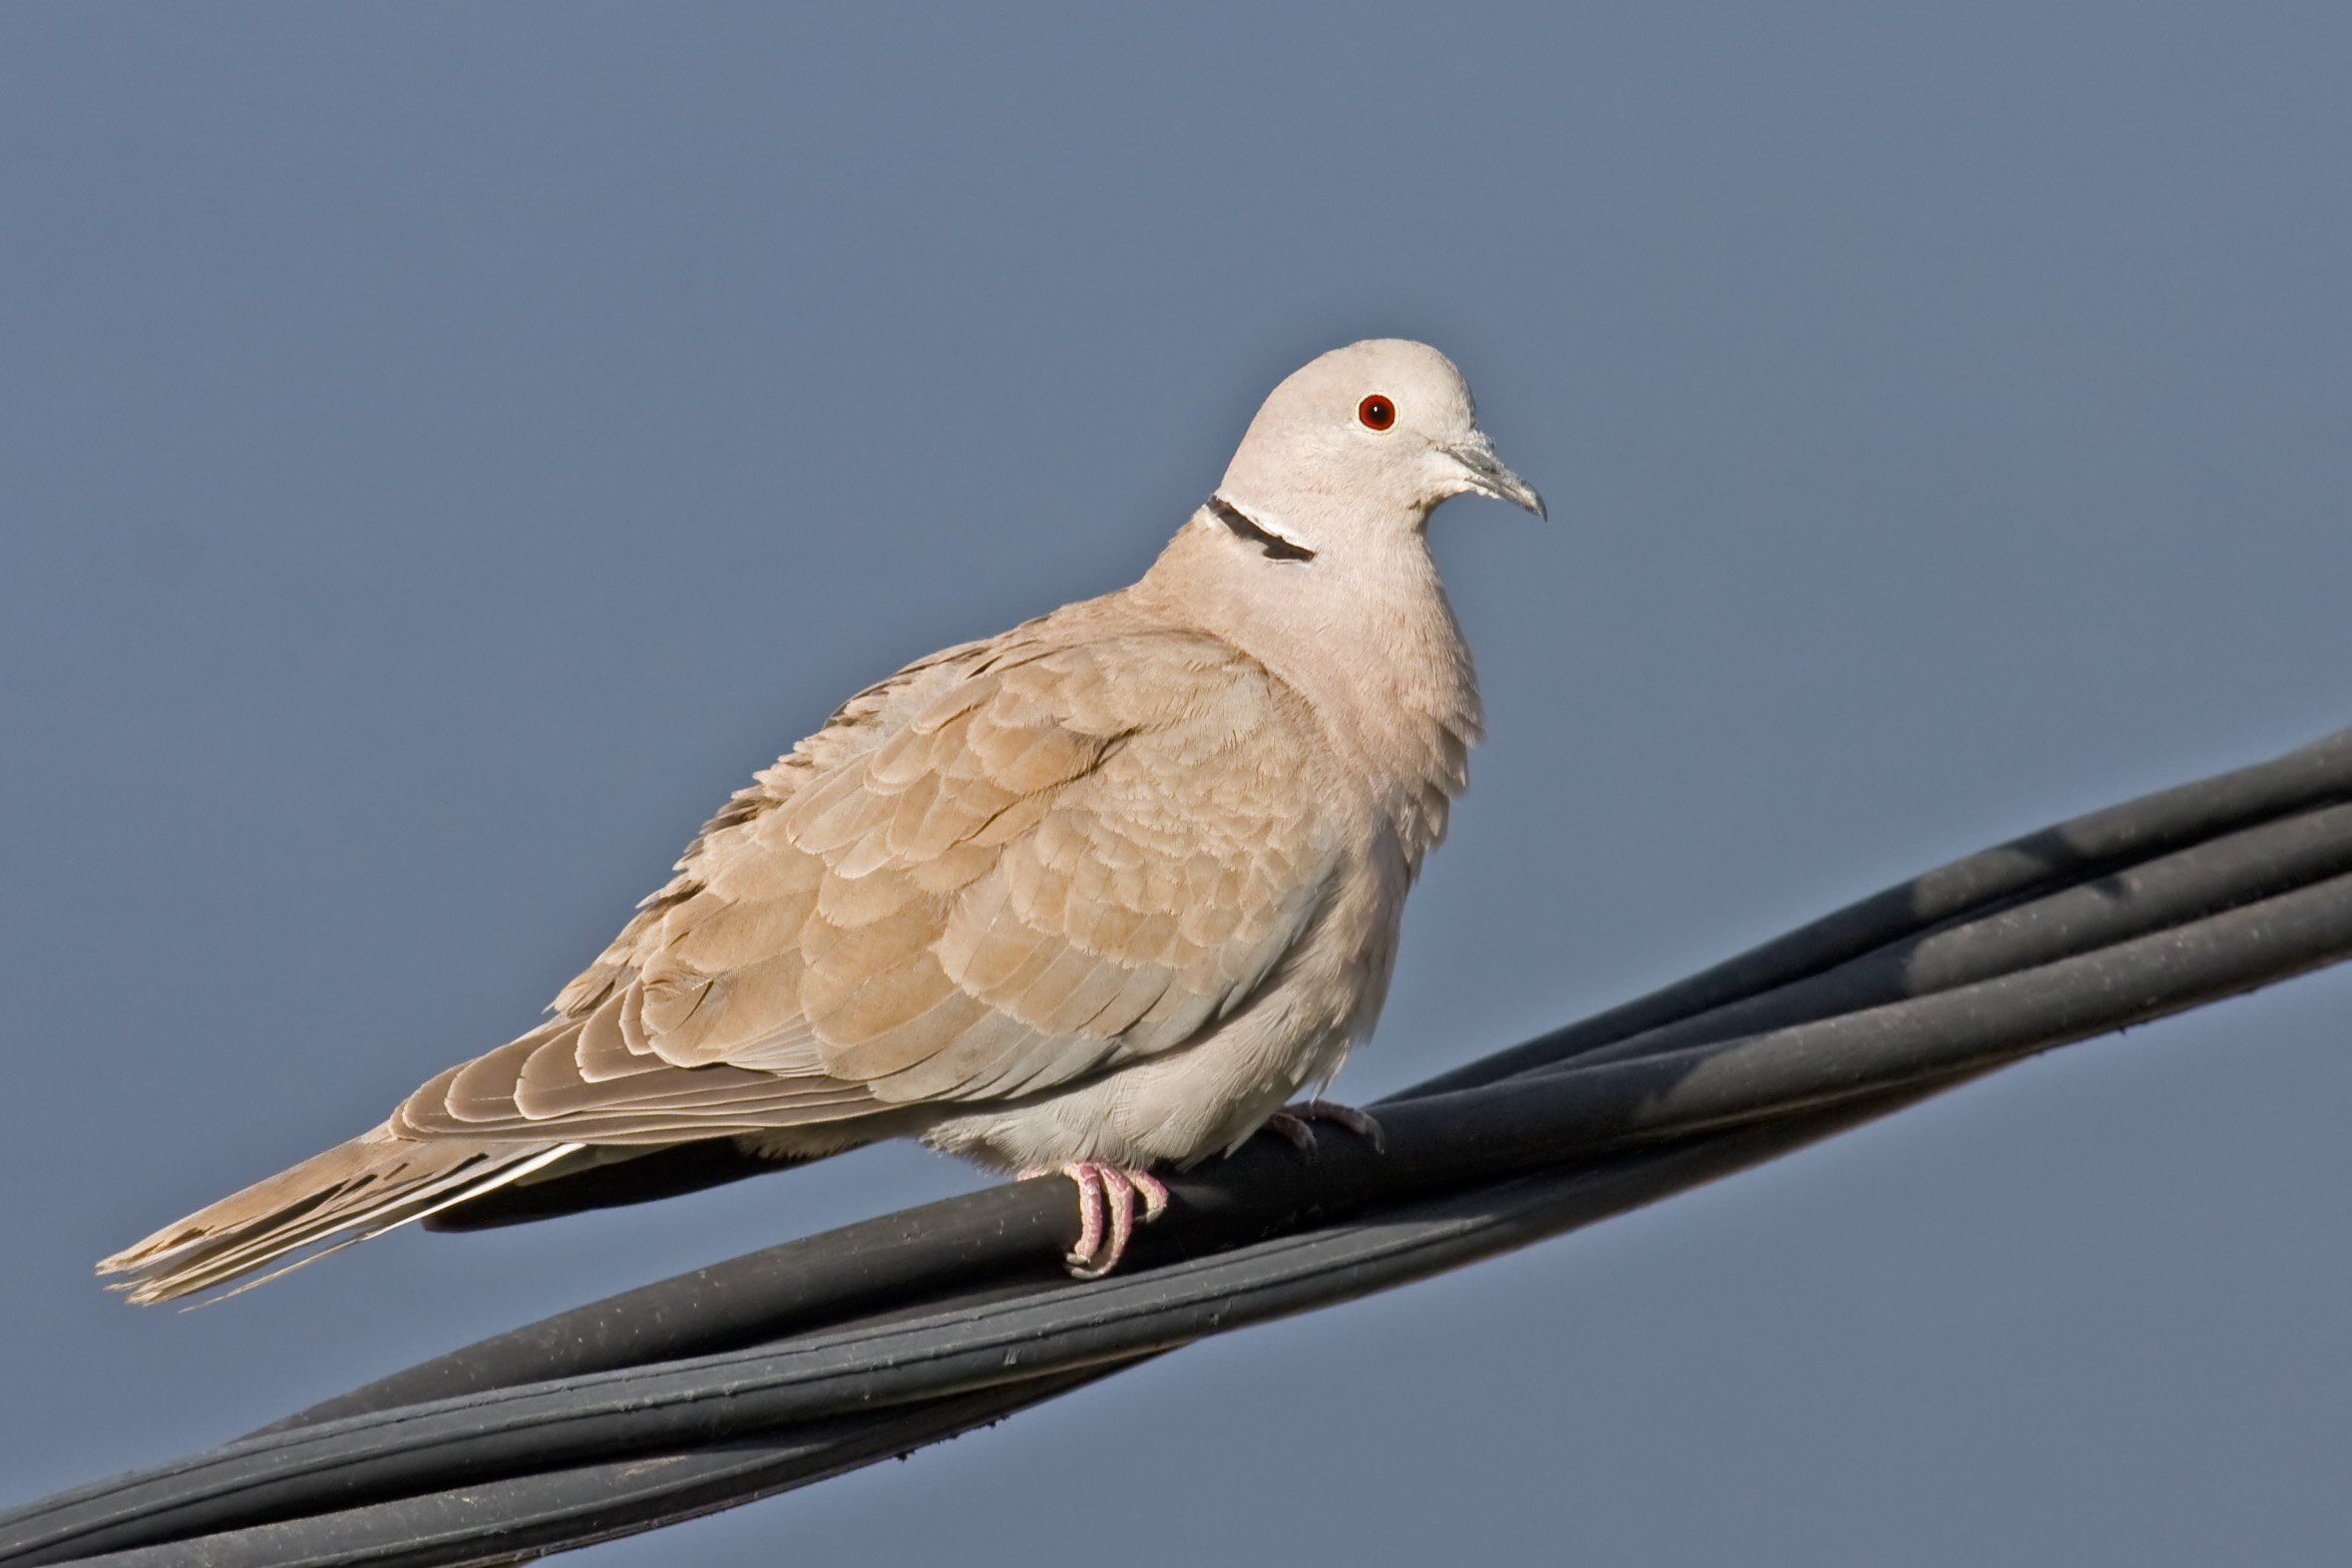
\includegraphics[width=0.7\textwidth,]{Collared_Dove.jpg}
	\end{figure}
	\blfootnote{You can also move the caption of a figure to the frame title or subtitle for a cleaner look.}
\end{frame}